\section{Aufbau}

Der Aufbau, der schematisch in Abbildung \autoref{aufbau} dargestell ist, besteht aus zwei Lasern, dem pump-Laser mit einer Wellenlänge von \SI{1047}{\nano\metre} und einem Fokus von \SI{20}{\micro\metre} und dem probe-Laser mit einer Wellenlänge von \SI{780}{\nano\metre} und einem Fokus von \SI{2}{\micro\metre}. Diese werden über Spiegel auf die Probe gerichtet, welche zwischen den Polen eines Magneten positioniert wird. Mit einer Kombination aus einem Glan-Thompson-Prisma und einem Lambda-Halbe-Filter kann die Intensität des pump-Lasers auf der Probe eingestellt werden. Für die optische Justage ist nach der Probe ein Objektiv mit 20-facher Vergrößerung, einer Linse und einem Mikroskop. Ein Wollaston-Prisma teilt den von der Probe kommenden probe-Laserstrahl auf zwei Photodioden auf, mit welcher  die Intensität gemessen wird, aus welcher die Reflektivität bestimmt wird.

Die Probe besteht aus einem Galliumarsenid-Substrat mit einem Galfenolfilm. An unterschiedlichen Stellen auf dem Film sind Gitterstrukturen verschiedener Höhen,  Breiten und Periodenlängen mit Ionenstrahlepitaxie eingebracht.

\section{Durchf\"{u}hrung}

Zur Messung der Gitterschwingungen wird ein pump-probe-Aufbau verwendet. Die durch die Oszillation der Gitterschwingungen hervorgerufene, periodische Reflektivitätsänderung wird bestimmt, indem die Intensität des von der Probe reflektierten probe-Laserstrahls mit einer Photodiode gemessen wird. Dazu wird der Aufbau zunächst einjustiert. Sowohl der pump-Laser, als auch der probe-Laser müssen auf die gleiche Stelle auf der Probe gerichtet sein. Das reflektierte Licht muss weiterhin auf eine Photodiode treffen.\par
Als erstes wird der Film ohne Höhenprofil angeregt und die Reflektivität gemessen. Daraus wird die Energiedissipation im Galfenol-Film bestimmt. Die Energiedissipation wird im Folgenden jeweils von jeder Messung als Untergrund subtrahiert. Es werden vier Gitter unterschiedlicher Tiefe vermessen. Für das tiefste Gitter wird außerdem eine Messung mit gedrehter Polarisation durchgeführt. Aus der Intensität wird die Oszillation der Reflektivitätsänderung der Probe bestimmt. Mit einer Fouriertransformation der Messwerte in der Zeitdomäne lassen sich Amplitude, Frequenz und Breite des Signals untersuchen.
\begin{figure}
  \centering
  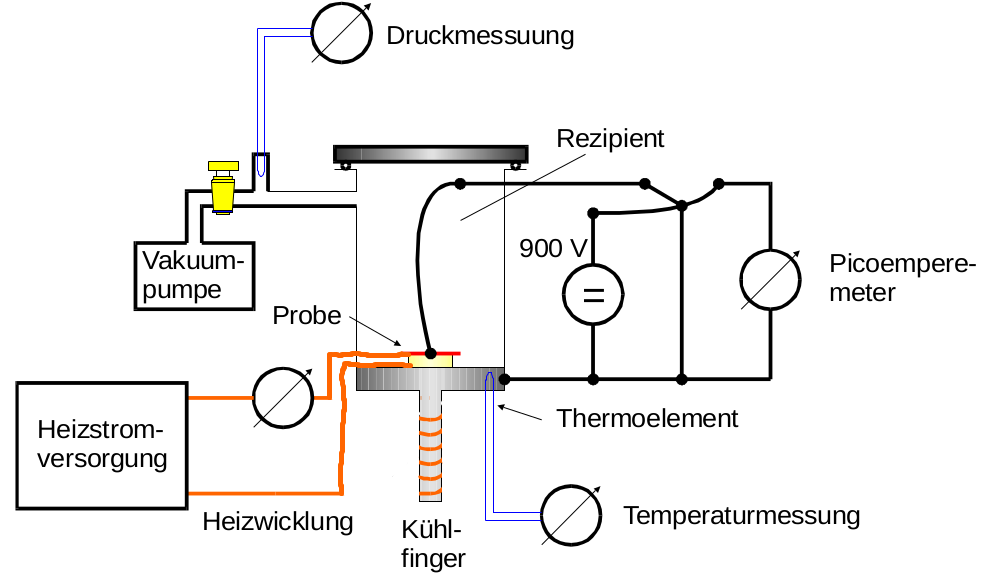
\includegraphics[width=0.75\textwidth]{img/aufbau.png}
  \caption{Schematischer Aufbau der Messapparatur \cite{FP}}
  \label{aufbau}
\end{figure}

\FloatBarrier
